\documentclass[english,11pt]{beamer}

\DeclareMathOperator{\Cov}{Cov}
\DeclareMathOperator{\Var}{Var}
\DeclareMathOperator{\E}{\mathbb{E}}
\DeclareMathOperator{\Proba}{\mathbb{P}}

\newcommand{\Covb}[2]{\ensuremath{\Cov\!\left[#1,#2\right]}}
\newcommand{\Eb}[1]{\ensuremath{\E\!\left[#1\right]}}
\newcommand{\Pb}[1]{\ensuremath{\Proba\!\left[#1\right]}}
\newcommand{\Varb}[1]{\ensuremath{\Var\!\left[#1\right]}}

% norm
\newcommand{\norm}[1]{\| #1 \|}

\newcommand{\indep}{\rotatebox[origin=c]{90}{$\models$}}





\usepackage{mathptmx,amsmath,amssymb,graphicx,bibentry,bbm,babel,ragged2e}

\makeatletter

\newcommand{\noun}[1]{\textsc{#1}}
\newcommand{\jitem}[1]{\item \begin{justify} #1 \end{justify} \vfill{}}
\newcommand{\sframe}[2]{\frame{\frametitle{#1} #2}}

\newenvironment{centercolumns}{\begin{columns}[c]}{\end{columns}}
%\newenvironment{jitem}{\begin{justify}\begin{itemize}}{\end{itemize}\end{justify}}









%\usetheme{Warsaw}
%\setbeamertemplate{footline}[text line]{}
%\setbeamercolor{structure}{fg=purple!50!blue, bg=purple!50!blue}
%\setbeamersize{text margin left=15pt,text margin right=15pt}




\usetheme{Boadilla}


% redefine palette
\definecolor{cybblue}{HTML}{1C6F91}


\setbeamercolor{structure}{fg=cybblue}

\setbeamercovered{transparent}


\addtobeamertemplate{title page}{%\hspace{-0.4cm}
\vspace{-0.8cm}
\hspace{-0.5cm}
%\includegraphics[height=1.2cm,width=1.2\textwidth]{template/bandeau3}\\
}{%
%\begin{textblock*}{150mm}(-1cm,-1.5cm)
%\end{textblock*}
}


\setbeamertemplate{footline}{
\hspace{0.2cm}
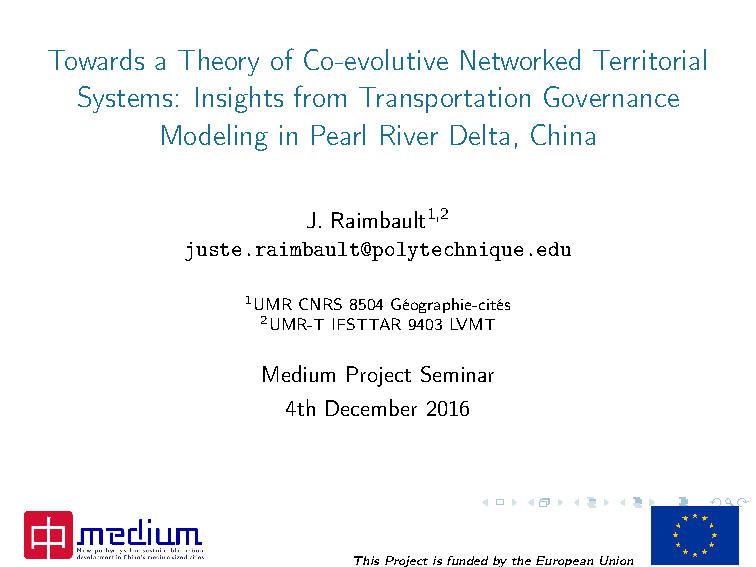
\includegraphics[height=0.75cm]{template/medium}
\hfill
\includegraphics[height=0.75cm]{template/eu}
\hspace{0.15cm}
\vspace{0.15cm}
}





\@ifundefined{showcaptionsetup}{}{%
 \PassOptionsToPackage{caption=false}{subfig}}
\usepackage{subfig}

\usepackage[utf8]{inputenc}
\usepackage[T1]{fontenc}


\usepackage[usenames,dvipsnames]{pstricks}
\usepackage{epsfig}



\makeatother

\begin{document}


\title{A Macro-scale Model of Co-evolution for Cities and Transportation Networks}

\author{J.~Raimbault$^{1,2}$\\
\texttt{juste.raimbault@polytechnique.edu}
}


\institute{$^{1}$UMR CNRS 8504 G{\'e}ographie-cit{\'e}s\\
$^{2}$UMR-T IFSTTAR 9403 LVMT\\
}


\date{Medium 2017 Conference\\\smallskip
Spatio-temporal Behavior in Complex Urban Systems\\\smallskip
17th June 2017
}


{


\setbeamertemplate{footline}{
\hspace{0.2cm}
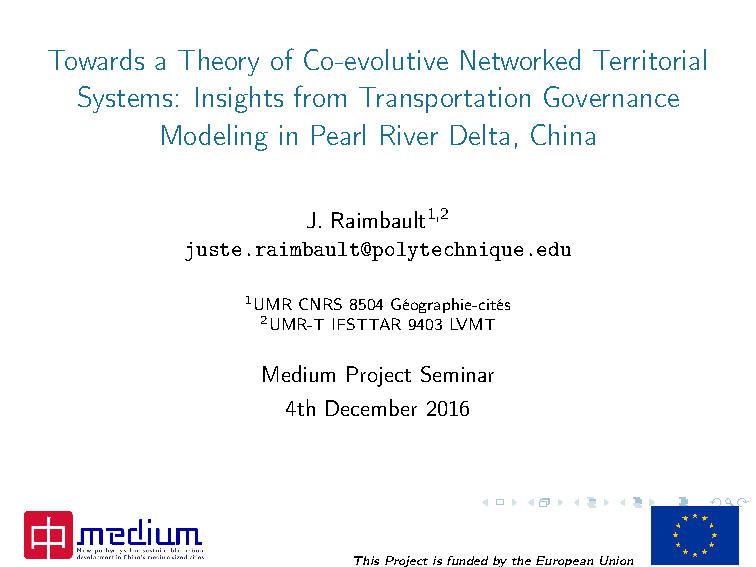
\includegraphics[height=1cm]{template/medium}
\hfill
\textit{This Project is funded by the European Union}\hspace{0.2cm}
\includegraphics[height=1cm]{template/eu}
\hspace{0.2cm}
\vspace{0.5cm}
}


\frame{\maketitle}

}




%%%%%%%%%%%%%%%%%%%
%% ABSTRACT

%The complexity of Urban Systems is closely linked to the co-evolutive character of their different components or agents (Pumain, 1997). In the case of cities and transportation networks, this co- evolution has been shown empirically (Bretagnolle, 2007) but remains poorly understood in terms of its dynamical processes. We introduce a model of spatial interactions between cities at the macro-scale, in the spirit of stochastic urban growth models inheriting from the Gibrat model (Favaro and Pumain, 2011). We include evolving transportation networks, in order to explore stylized hypothesis on the interactions and drivers of the growth of both network and cities. In a multi-modeling fashion, the model can take into account various processes such as between cities direct interactions, network-mediated interactions, feedback of network flows, and for the network demand-induced growth. The latter is tested at different abstraction levels that are the time-distance matrix between cities, and physical network growth trying to satisfy greedy time-gain optimization criteria. We use as a benchmark network the geographical shortest paths that have been shown in a previous work to already capture network effects (Raimbault, 2016). The model is tested and explored on synthetic city systems, generated following a simple heuristic to follow the rank-size law and Central Place Theory. The systematic exploration through intensive computation unveils different interaction regimes accross the parameter space. In some, the introduction of the network can drastically change the fate of some cities, whereas the top-distribution hierarchy is reinforced, what is consistent with empirical observations in the literature. Some regimes actually exhibit circular causalities between network and city growth, corresponding to the intricated co-evolution. The model will be applied to the French Urban System on long time dynamical data (Pumain-INED database for populations spanning between 1831 and 1999, with the evolving railway network from 1850 to 2000, and a specifically-designed database of the highway networks containing its full genesis from 1950 to 2015), and to the Chinese Urban System after 2000 with the High Speed Rail (HSR) network, both realized and planned. Expected results concern both accurate city population growth reproduction, and network patterns, i.e. how does taking into account dynamical networks can introduce further exploratory power in such models, and reciprocally how can such coupled models produce realistic networks compared to more classical autonomous models of network growth. The role of medium-sized cities on the trajectories of the system can also be examined with the model. Finally, a comparison between the urban systems in different geographical and political contexts and at different scales should unveil implications of planning on the interactions between networks and cities, for example by comparing the rather bottom-up growth of the French railway network to the top-down state-planned French highway and Chinese HSR networks.




%%%%%%%%%%%%%%%%%%%
\section{Introduction}
%%%%%%%%%%%%%%%%%%%


\sframe{Systems of Cities and Transportation Networks}{

\centering

% -> picture of HK-Zh-Macao bridge

%{\tiny Source : Wikipedia}

}


\sframe{Co-evolution}{

% what is the co-evolution, why model it, what model exist

}


\sframe{Research Objective}{

% question / objective

% incl. schema on what is a strongly coupled co-evolutive model

}




%%%%%%%%%%%%%%%%%%%
\section{Model and Results}
%%%%%%%%%%%%%%%%%%%


\sframe{Model : Rationale}{
  % - explain choices, funding literature etc.
  % - considerations on randomness ; comparison with Simpopnet
}

\sframe{Generic Model}{

}

\sframe{Model : Abstract Network}{

}

\sframe{Model : Physical Network}{

}


%  Results
%   - at least one illustration of each ?
%   - variability within one run
%   - synthetic virtual : at least two stunning facts
%         * causality regimes ?
%         * complexity/diversity of trajs
%   - synthetic physical : a first lesson ?

% - a summary slide with "take home message" of results

\sframe{Results}{

}



%%%%%%%%%%%%%%%%%%%
\section{Future Applications}
%%%%%%%%%%%%%%%%%%%


\sframe{Case studies}{

}





\sframe{Conclusion}{

% Discussion and Conclusion

$\rightarrow$ 

\medskip

$\rightarrow$ 

\bigskip
\bigskip
\bigskip


\footnotesize{ - All code and data available at \texttt{https://github.com/JusteRaimbault/CityNetwork/tree/master/Models/MacroCoevol}

}

}




\sframe{Reserve slides}{

\centering

\Large

\textbf{Reserve Slides}

}

\sframe{Model Formalization : Interactions}{

}

\sframe{Model Formalization : Network Growth}{

}







%%%%%%%%%%%%%%%%%%%%%
\begin{frame}[allowframebreaks]
\frametitle{References}
\bibliographystyle{apalike}
\bibliography{/Users/Juste/Documents/ComplexSystems/CityNetwork/Biblio/Bibtex/CityNetwork}
\end{frame}
%%%%%%%%%%%%%%%%%%%%%%%%%%%%






\end{document}







